
\section{Counting with digit regions}


\begin{figure}[H]
    \centering
    \begin{subfigure}[t]{0.43\textwidth}
        \centering
        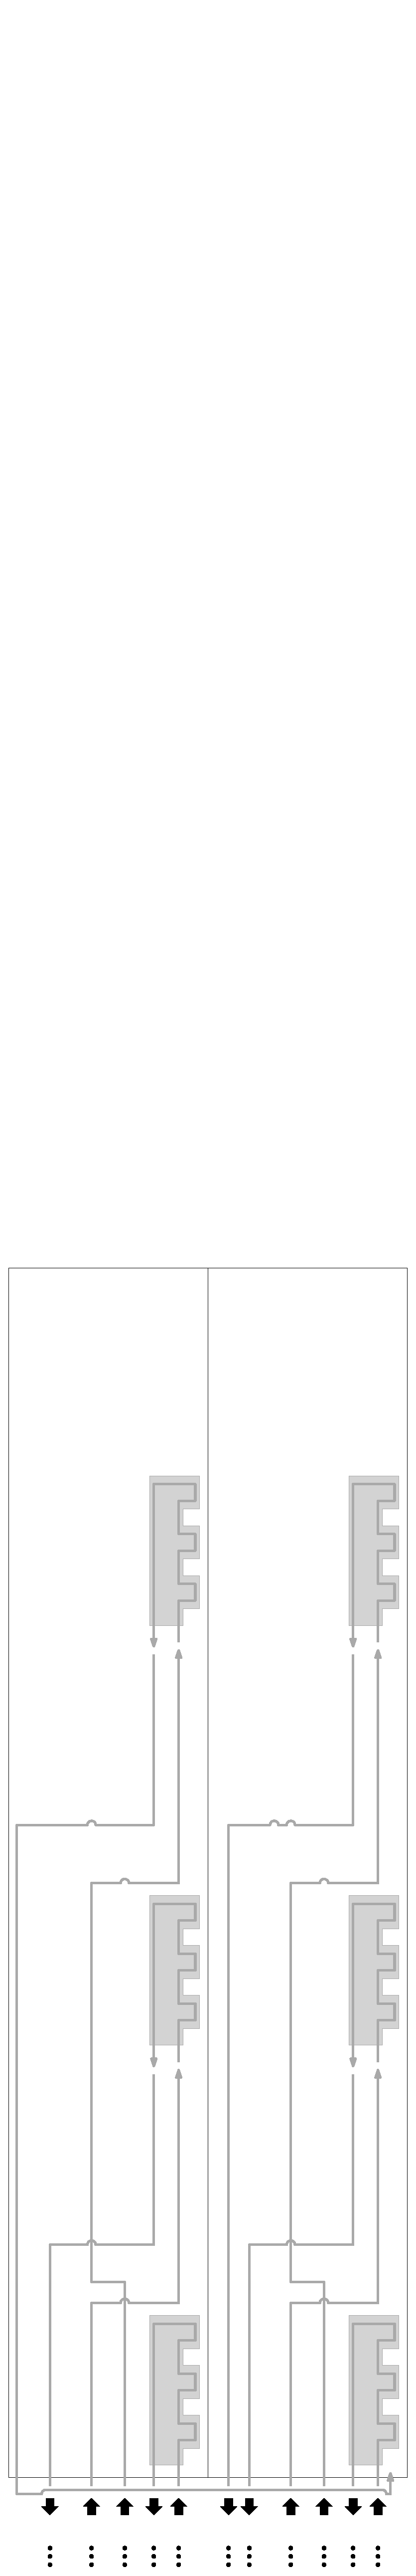
\includegraphics[width=0.43\textwidth]{counter_read_start_general_case3_middle_level}
        \caption{\label{fig:counter_read_start_case3_middle_level} A ``clean'' counter row, before any reading has started.}
    \end{subfigure}%
    ~
    \begin{subfigure}[t]{0.43\textwidth}
        \centering
        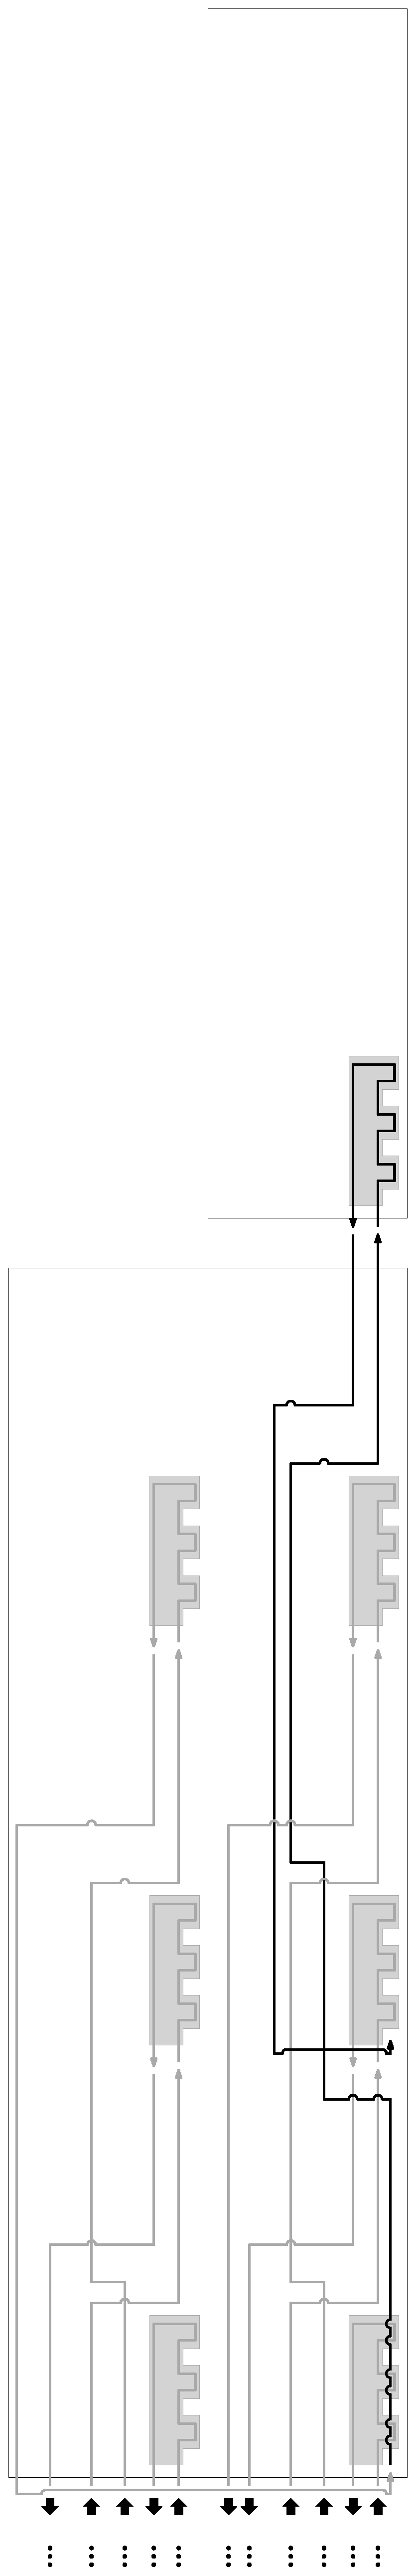
\includegraphics[width=0.43\textwidth]{counter_read_digit1_return_read_digit2_general_case3_middle_level}
        \caption{\label{fig:counter_read_digit1_general_case3_middle_level} Read digit 1 in the current row, write digit 1 in the next row.}
    \end{subfigure}%
    ~
\end{figure}
\begin{figure}[H]\ContinuedFloat
    \centering
    \begin{subfigure}[t]{0.43\textwidth}
        \centering
        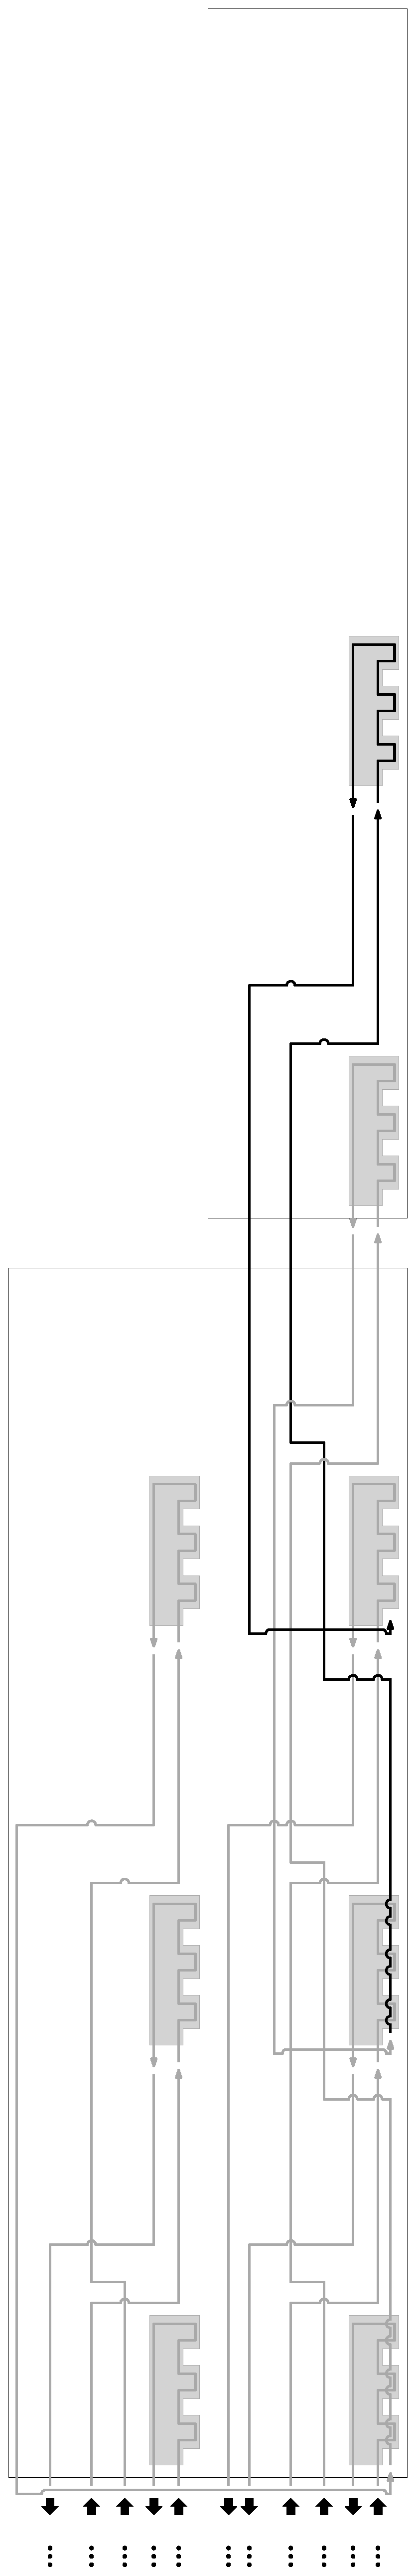
\includegraphics[width=0.43\textwidth]{counter_read_digit2_return_read_digit3_general_case3_middle_level}
        \caption{\label{fig:counter_read_digit2_general_case3_middle_level} Read digit 2 in the current row, write digit 2 in the next row.}
    \end{subfigure}%
    ~
    \begin{subfigure}[t]{0.43\textwidth}
        \centering
        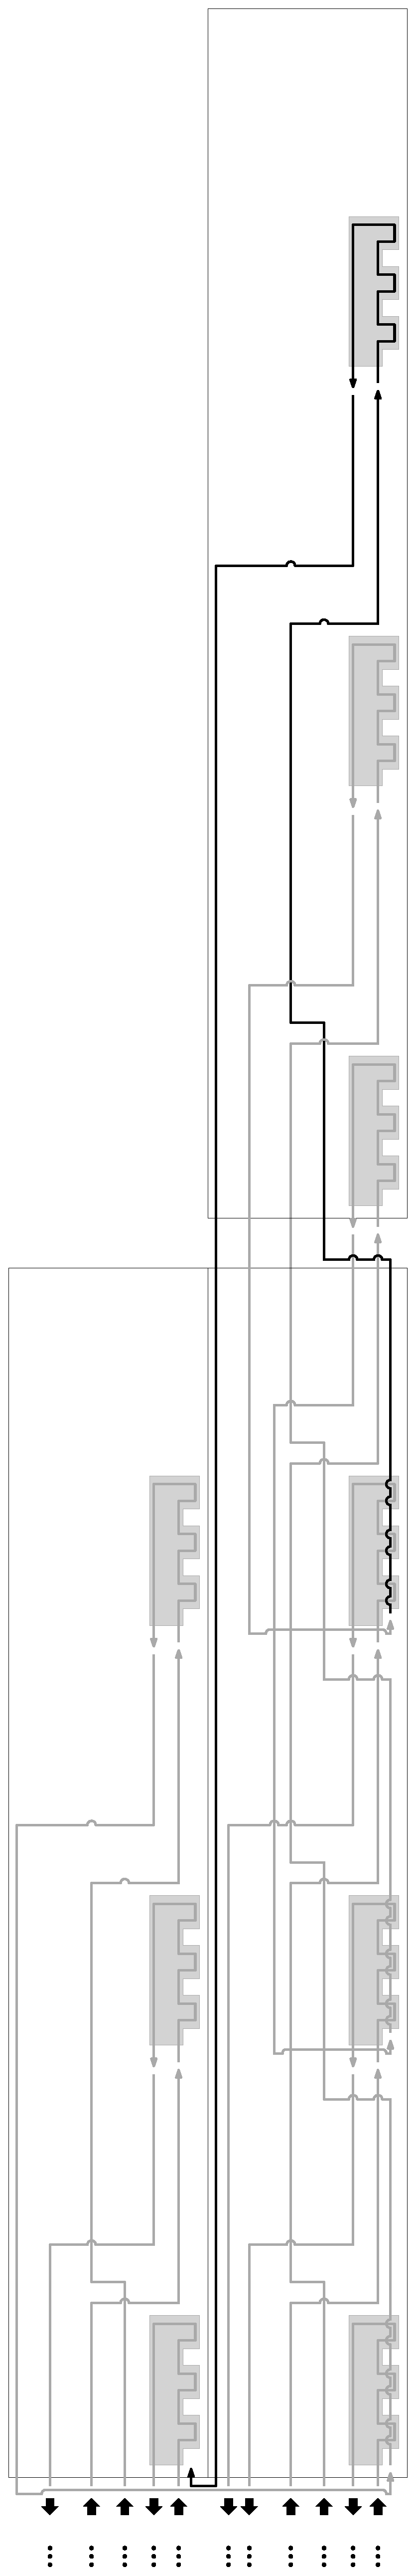
\includegraphics[width=0.43\textwidth]{counter_read_digit3_return_read_digit1_general_case3_middle_level}
        \caption{\label{fig:counter_read_digit3_general_case3_middle_level} Read digit 3 in the current row, write digit 3 in the next row.}
    \end{subfigure}%
    ~

\end{figure}
\begin{figure}[H]\ContinuedFloat
    \caption{\label{fig:counter_read_digit_return_read_digit_general_case3}
    This illustrates how a counter reads and writes a digit region, in a general sense.
    The counter starts in the rightmost digit region by reading the bottommost digit within
    that region. After reading digit 1 in the current row, the corresponding digit region in
    the next row be started in the next row. The counter writes the first digit in the next
    row, and then returns to the second digit in the current digit region.
    Once all the digits in the current digit region are read and written into the next row,
    the counter can then do one of the following: continue reading digits by moving on to the
    next digit region, cross back all the way to the right of the rectangle and start reading
    the next row, or halt.}
\end{figure}

\subsection{Digit regions}

Each logical row of the counter is made up of $\ceil*{\frac{d}{3}}$ ``digit regions".
%
A digit region is a group of 1-3 digits, stacked vertically on top of one another.
%
Within a digit region, the digits are sorted in order of significance, thus the top digit is the most signifcant digit, the middle digit
is second most significant and the bottommost digit is the least signifcant.
%
The leftmost digit region is most signifcant and the rightmost is the least signifcant.
%

The counter reads digit 1 in the rightmost digit region, then writes digit $1^\prime$ in the digit region directly north in the next row.
%
After writing this first digit, the counter returns back to the current row and reads digit 2.
%
Upon reading digit 2 in the current row, it then writes digit $2^\prime$ in the next row and returns to the current row.
%
Finally, in the current row, it reads digit 3, the last digit remaining, and writes digit $3^\prime$ in the next row.
%
Now that all three digits in this digit region have been evaluated, the counter will repeat this process for all remaining digit regions in the current row.
%

In the last digit region, which we will refer to as the MSR (most significant region), the region may or may not contain all 3 digits like the earlier regions.
%
Because of this, there are three cases we must account for: case 1 if the MSR only has one digit; case 2 if the MSR only has two digits; or case 3 if the MSR has three digits.
%

%
In case 1, the MSR adds an additional 2 tiles to the overall width of the rectangle.
%
In case 2, the MSR adds an additional 4 tiles to the overall width of the rectangle.
%
And, similar to all regular digit regions with 3 digits, in case 3 the MSR adds an additional 6 tiles to the overall width of the rectangle.
%
As a result of these cases, we're able to utilize these different to fine tune the width of the rectangle such that we only need one filler tile in the event that $k$ is odd.
%


\begin{figure}[H]
    \centering
    \caption{\label{fig:comparison_of_digits_in_different_counters}Digits in a typical counter vs. digits separated into digit regions.}
    \begin{subfigure}[t]{0.49\textwidth}
        \centering
        
\includegraphics[width=2in]{digits_normal_counter}
        \caption{\label{fig:digits_normal_counter} Digits in a typical counter.}
    \end{subfigure}%
    ~
    \begin{subfigure}[t]{0.49\textwidth}
        \centering
        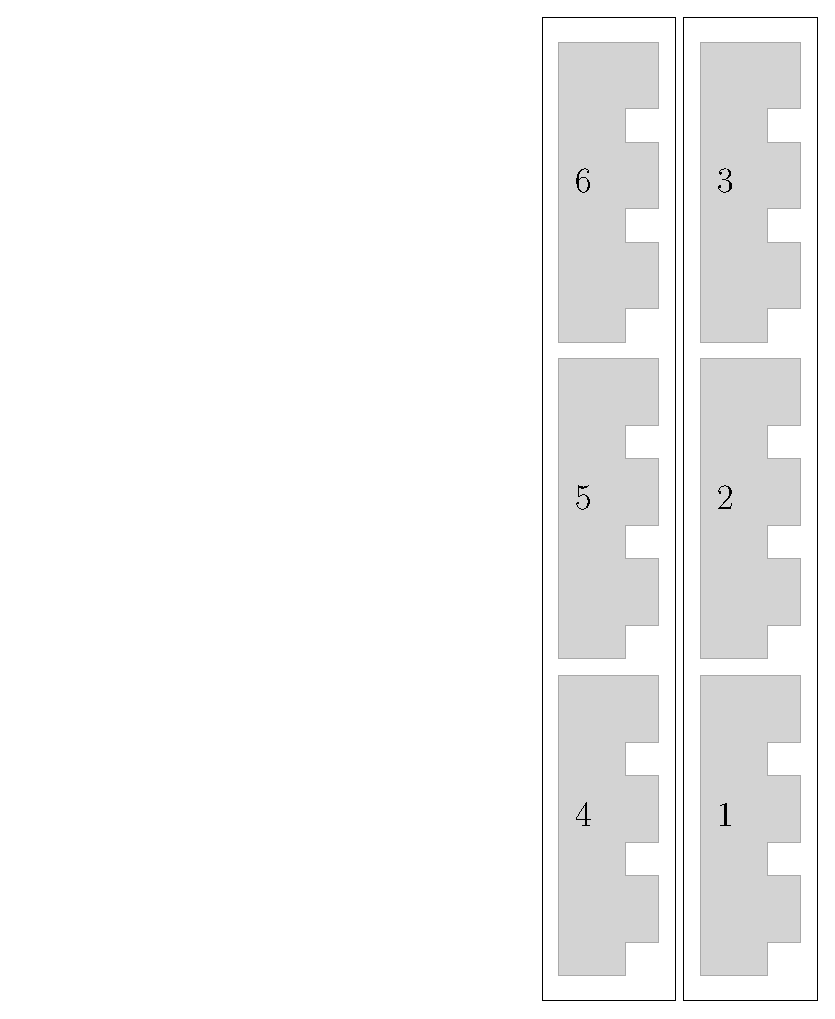
\includegraphics[width=2in]{digits_digit_region_counter}
        \caption{\label{fig:digits_digit_region_counter} Digits in two digit regions, stacked vertically.
        Digits 1-3 are in digit region 1, and digits 4-6 are in digit region 2.}
    \end{subfigure}%
    ~
\end{figure}

Contrary to a typical counter, each counter row has an approximate height of 3 digits $\approx 12l$.
The digits are stacked up to 3, once a digit region is full, we add another digit region to the left, and repeat.

\subsection{Detecting the edges}

The counter must detect if a digit is in the MSR and if it's in the MSR, whether or not it is the most
signifcant digit. To do this, all digits are encoded with two additional bits on the least signifcant end.
If bit 0 is 1, the reader tiles know they could be reading the most signifcant digit (MSD) or in case 2, the
second most signifcant digit. If bit 1 is 1, the digit currently being read is the MSD, otherwise
the digit is digit 1 in case 2.

\begin{table}[H]
    \begin{tabular}{|l|l|l|}
    \hline
        bit$_1$ & bit$_0$ & Meaning                                \\ \hline
            0   & 0       & digit is not in MSR                    \\ \hline
            0   & 1       & digit is in the MSR but is not the MSD \\ \hline
            1   & 0       &                                        \\ \hline
            1   & 1       & digit is in the MSR and is MSD         \\ \hline
    \end{tabular}
\end{table}